\tableofcontents
\clearpage

\section{Индивидуальное задание}

Выбрать пять музыкальных произведений различных композиторов и жанров. Произведение должно быть доступно в формате midi. Используя код Проекта 6 получить по две визуализации для каждого музыкального произведения.

\section{Полученные графы}

Ниже представлены графы, полученные в результате визуализации различных музыкальных произведений. В качестве музыкальных произведений были выбраны стандартные рингтоны и звуки iphone.

\begin{figure}[H]
	\caption{Граф 1 night-owl}
	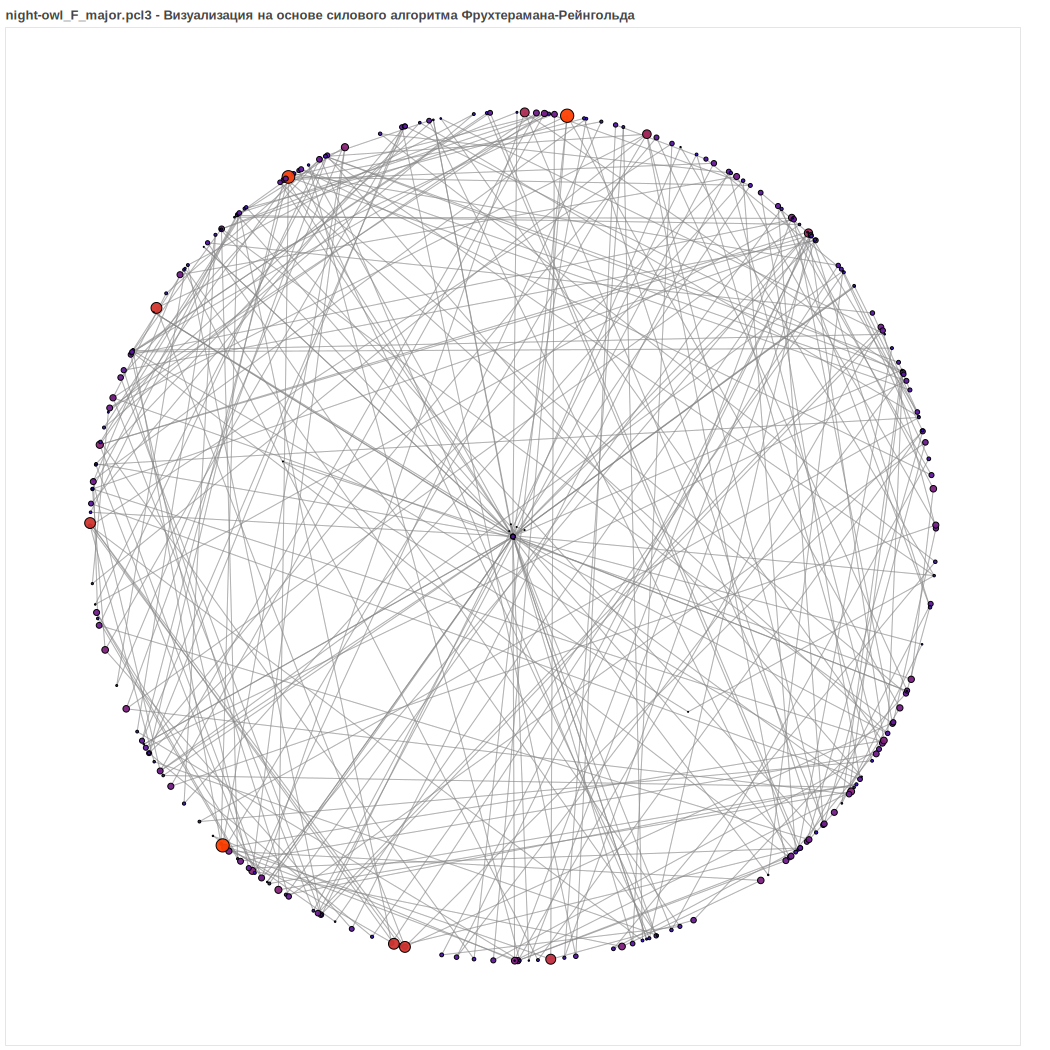
\includegraphics[width=0.9\textwidth]{img/night-owl1.pdf}
\end{figure}

\begin{figure}[H]
	\caption{Граф 2 night-owl}
	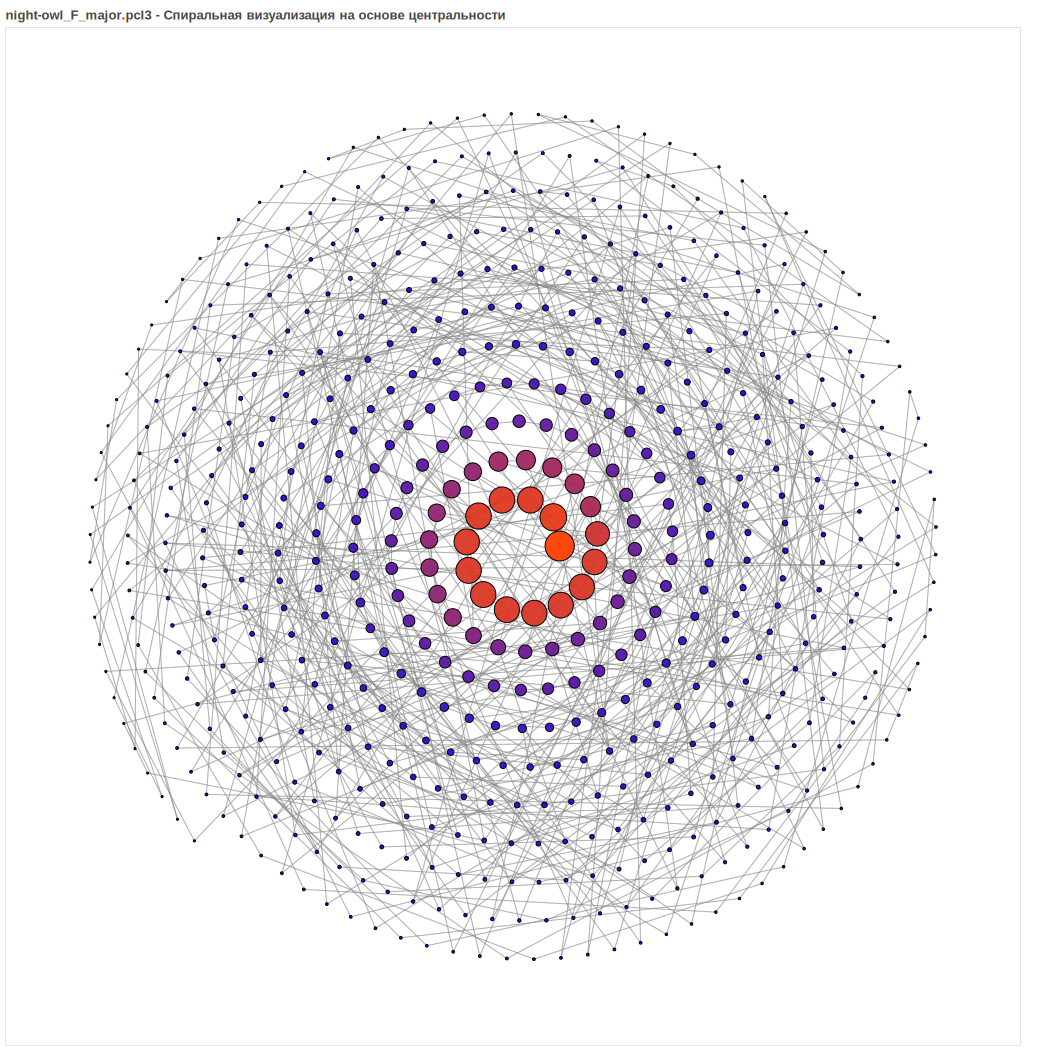
\includegraphics[width=0.9\textwidth]{img/night-owl2.pdf}
\end{figure}

\begin{figure}[H]
	\caption{Граф 1 radiate}
	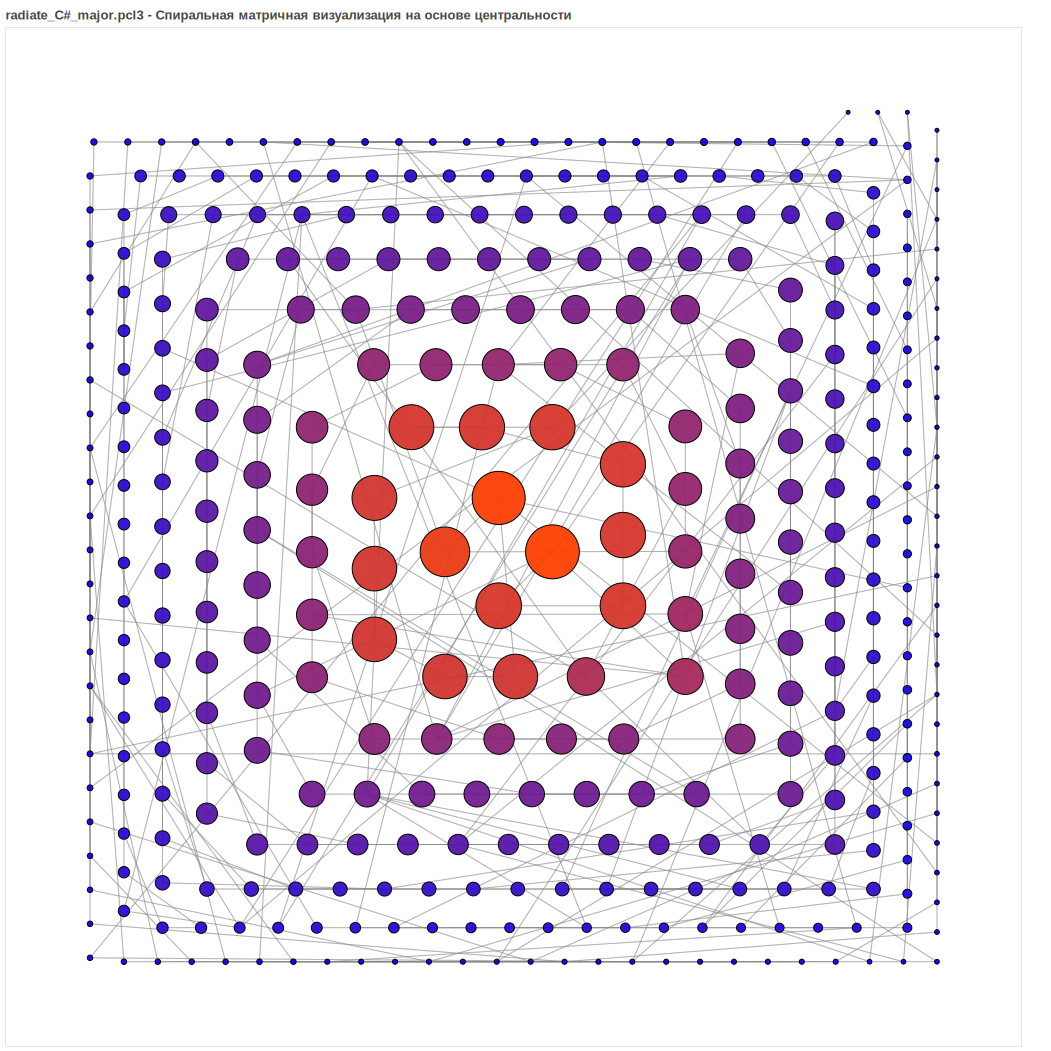
\includegraphics[width=0.9\textwidth]{img/radiate1.pdf}
\end{figure}

\begin{figure}[H]
	\caption{Граф 2 radiate}
	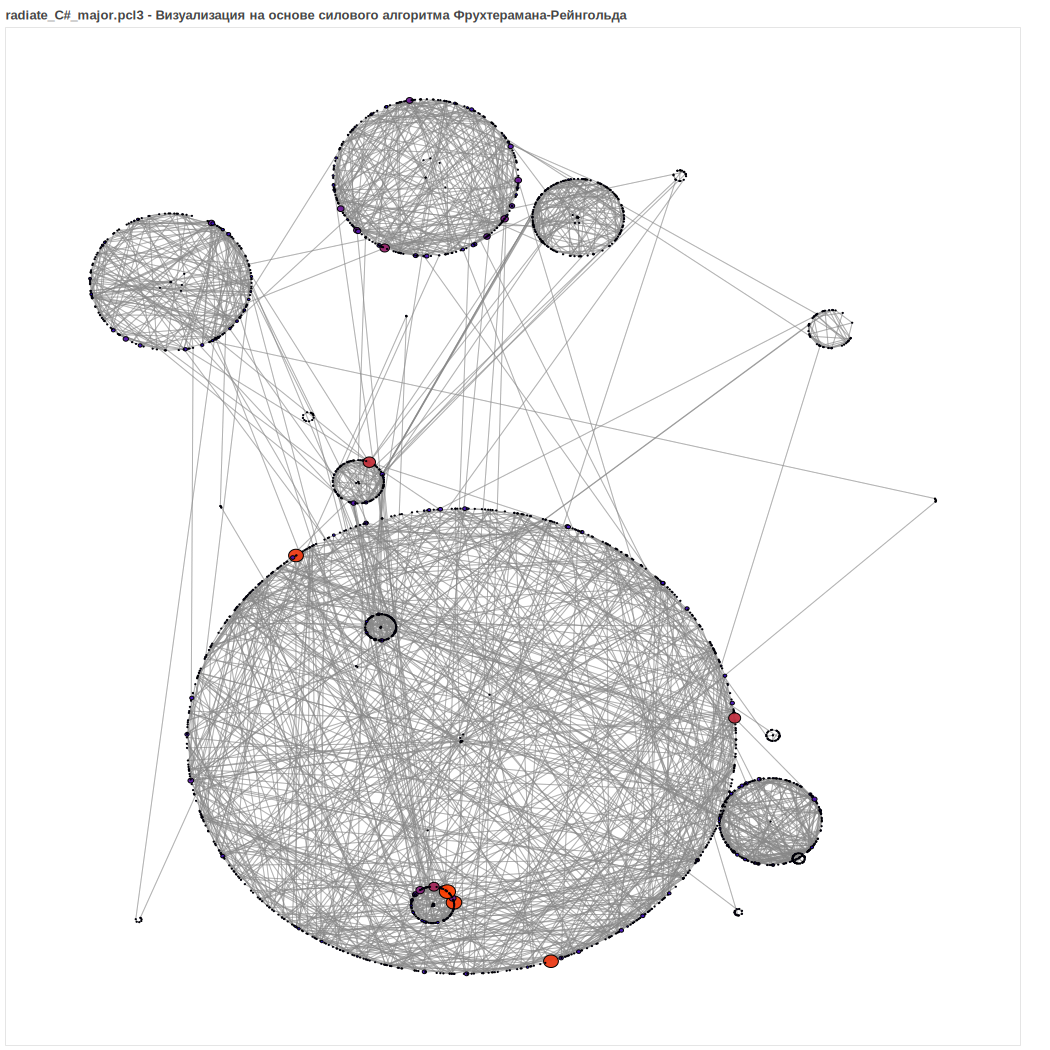
\includegraphics[width=0.9\textwidth]{img/radiate2.pdf}
\end{figure}

\begin{figure}[H]
	\caption{Граф 1 ringtone}
	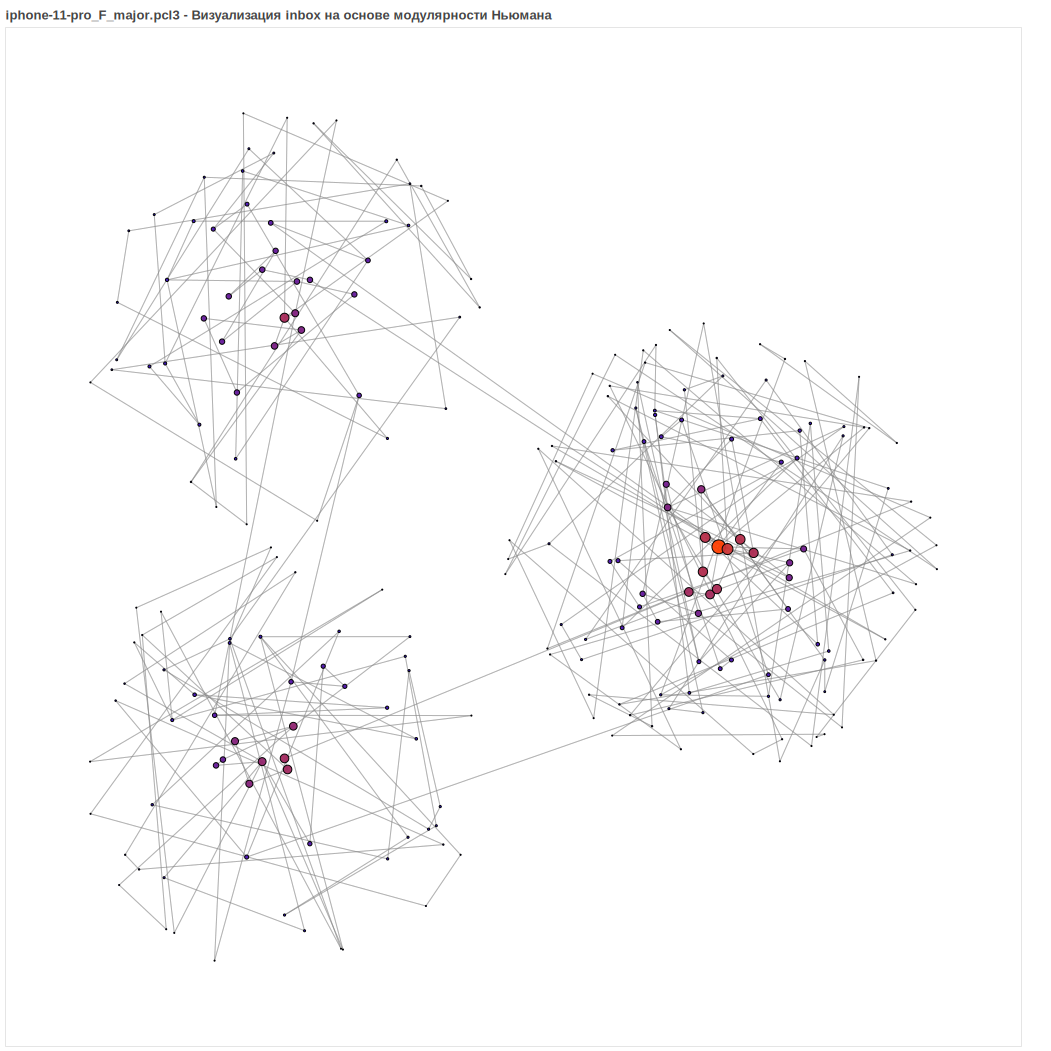
\includegraphics[width=0.9\textwidth]{img/ringtone1.pdf}
\end{figure}

\begin{figure}[H]
	\caption{Граф 2 ringtone}
	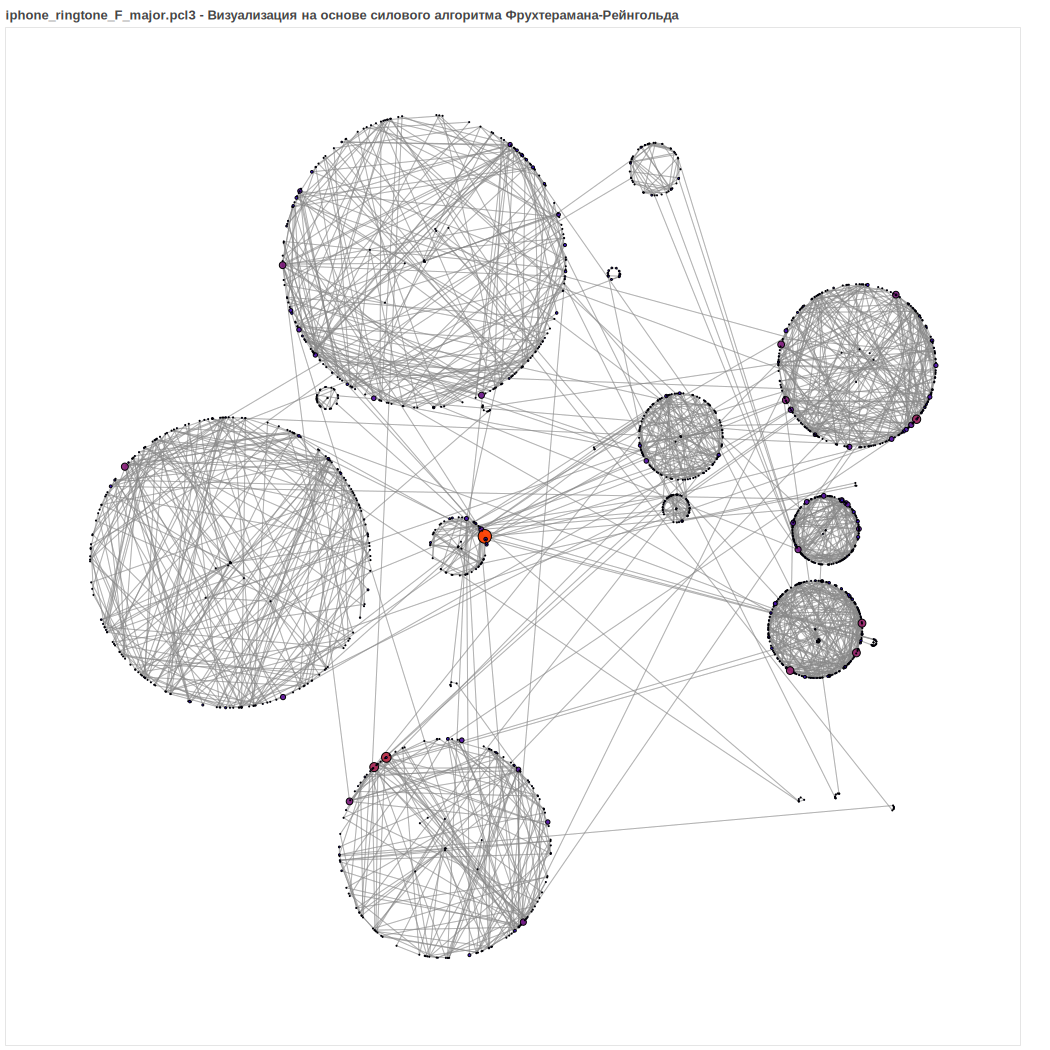
\includegraphics[width=0.9\textwidth]{img/ringtone2.pdf}
\end{figure}

\begin{figure}[H]
	\caption{Граф 1 silk}
	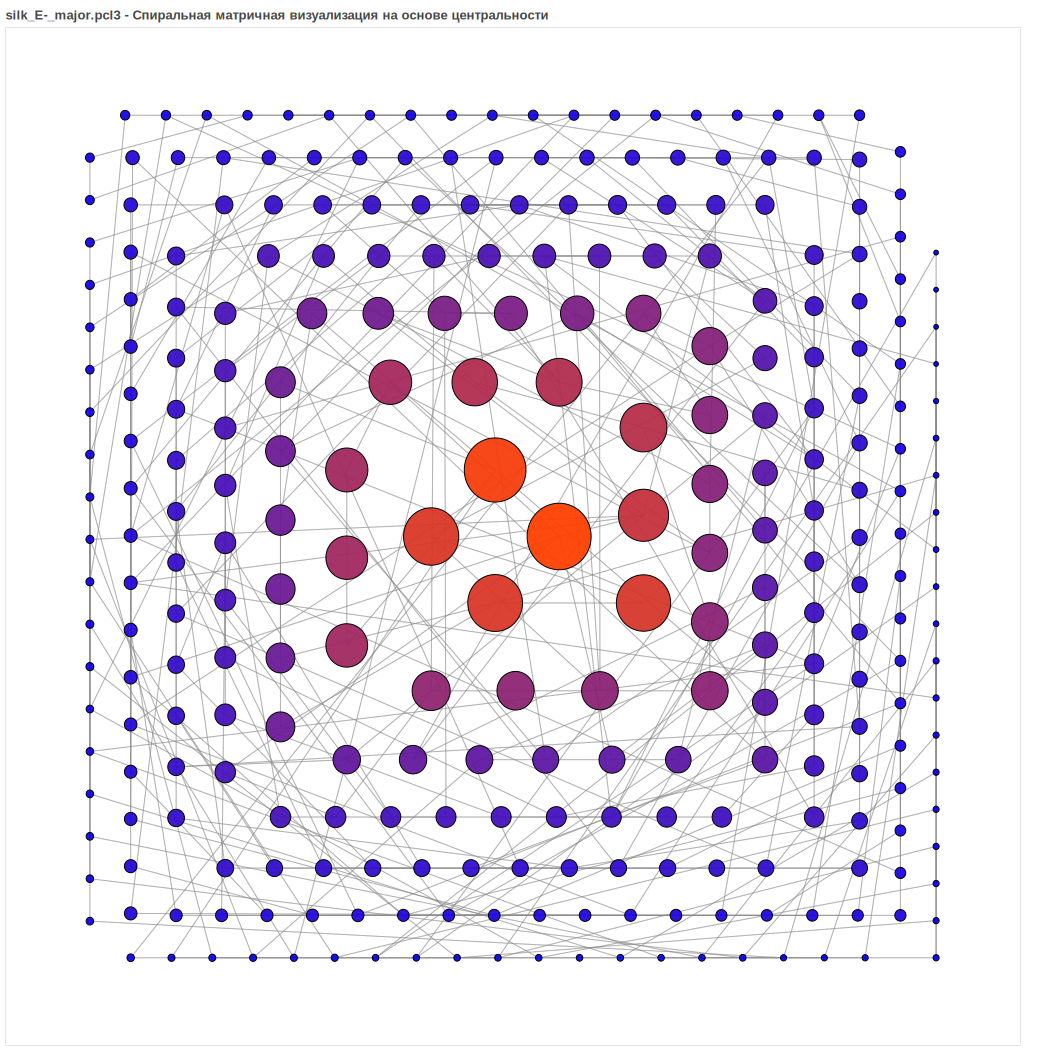
\includegraphics[width=0.9\textwidth]{img/silk1.pdf}
\end{figure}

\begin{figure}[H]
	\caption{Граф 2 silk}
	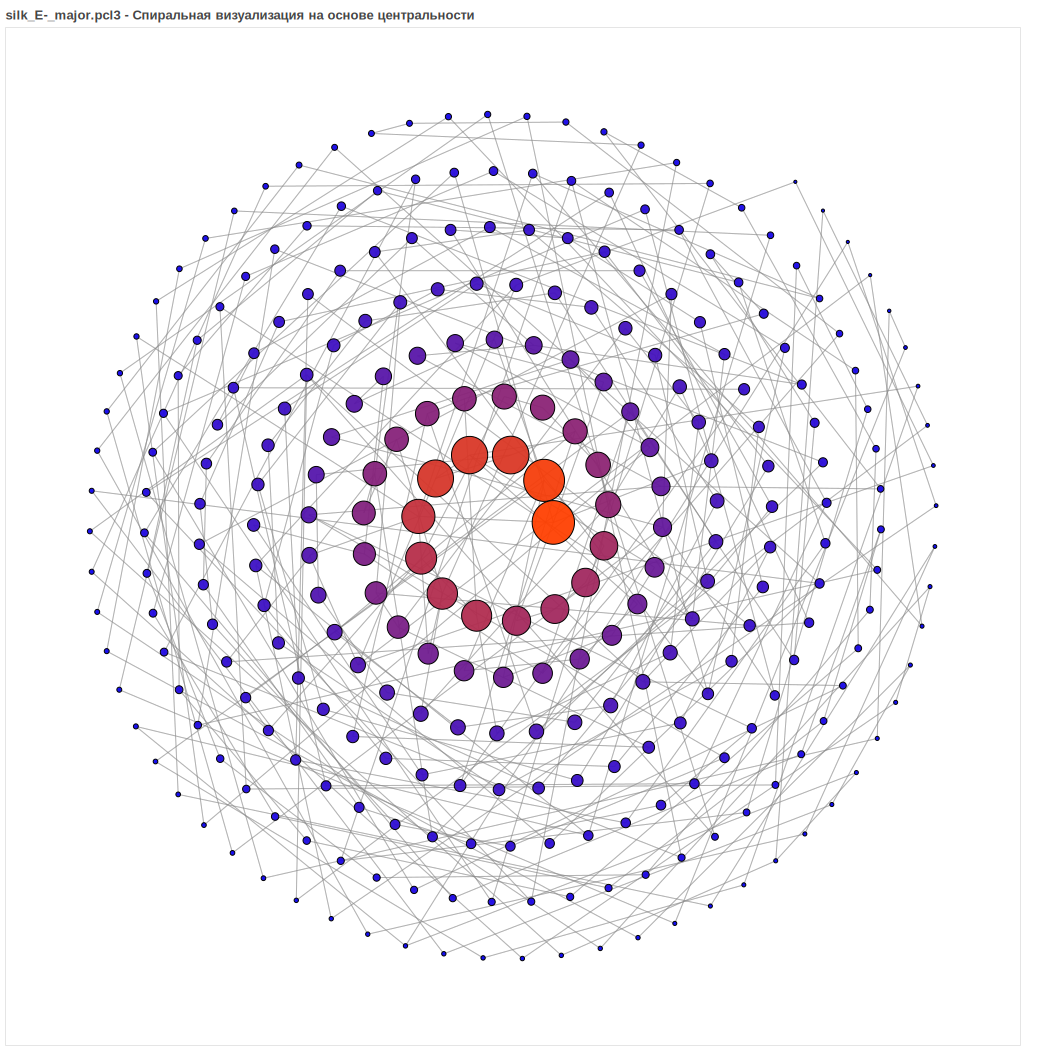
\includegraphics[width=0.9\textwidth]{img/silk2.pdf}
\end{figure}

\begin{figure}[H]
	\caption{Граф 1 waves}
	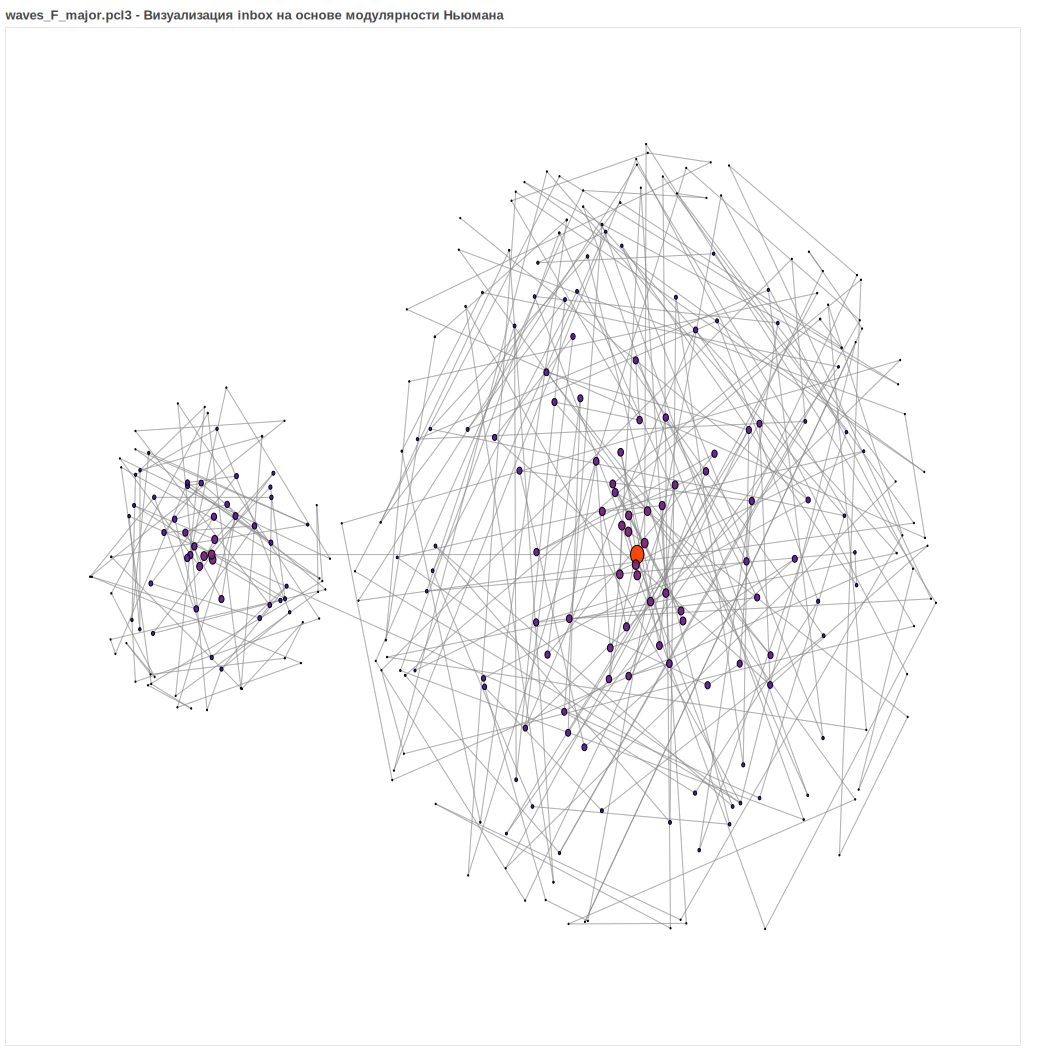
\includegraphics[width=0.9\textwidth]{img/waves1.pdf}
\end{figure}

\begin{figure}[H]
	\caption{Граф 2 waves}
	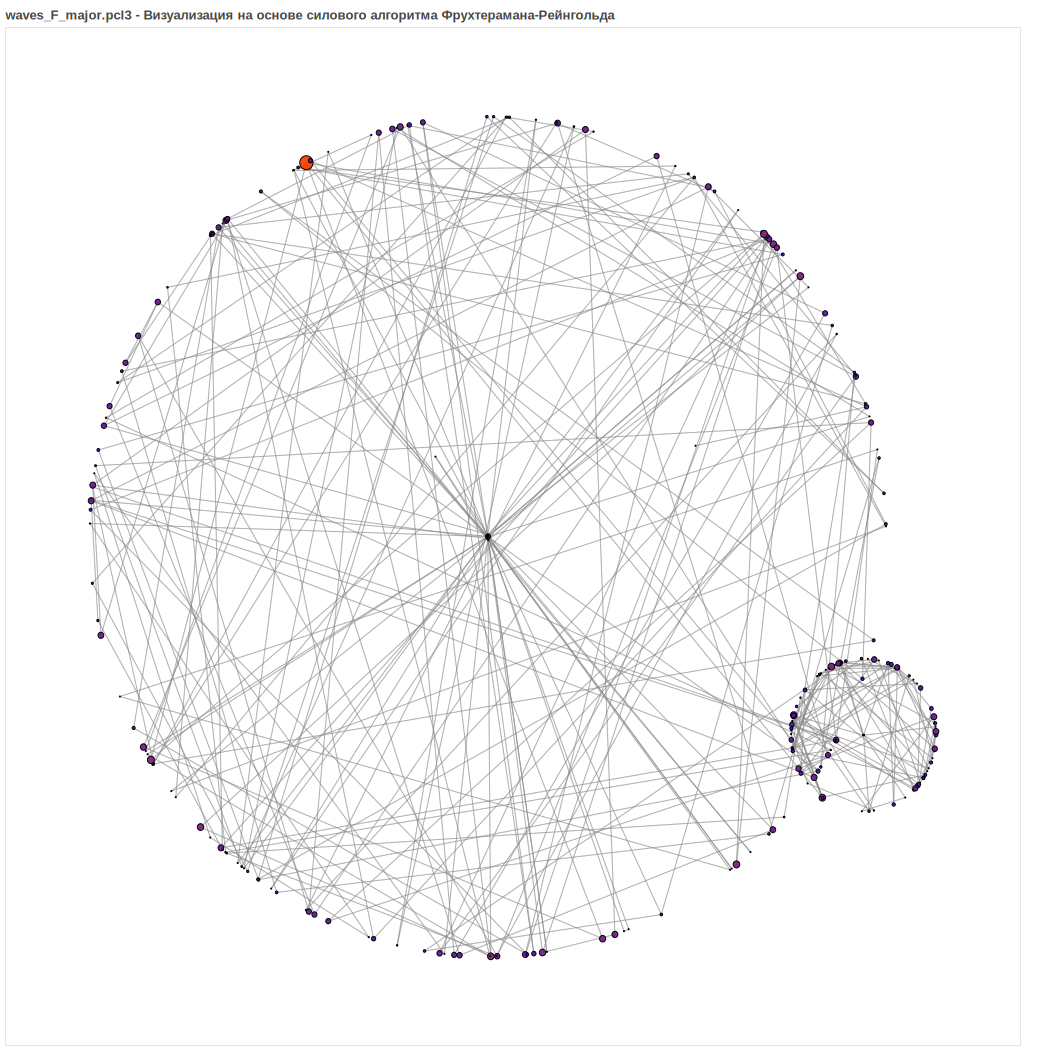
\includegraphics[width=0.9\textwidth]{img/waves2.pdf}
\end{figure}

\section{Полученные изображения}

Ниже представлены изображения, полученные с помощью нейросети, путем объединения графов выше и фотографии времени года. Изображения представлены по порядку с января по декабрь.

\begin{figure}[H]
	\caption{Визуализация января}
	\includegraphics[width=0.9\textwidth]{img/jan.jpeg}
\end{figure}

\begin{figure}[H]
	\caption{Визуализация февраля}
	\includegraphics[width=0.9\textwidth]{img/feb.jpeg}
\end{figure}

\begin{figure}[H]
	\caption{Визуализация марта}
	\includegraphics[width=0.9\textwidth]{img/mar.jpeg}
\end{figure}

\begin{figure}[H]
	\caption{Визуализация апреля}
	\includegraphics[width=0.9\textwidth]{img/apr.jpeg}
\end{figure}

\begin{figure}[H]
	\caption{Визуализация мая}
	\includegraphics[width=0.9\textwidth]{img/may.jpeg}
\end{figure}

\begin{figure}[H]
	\caption{Визуализация июня}
	\includegraphics[width=0.9\textwidth]{img/jun.jpeg}
\end{figure}

\begin{figure}[H]
	\caption{Визуализация июля}
	\includegraphics[width=0.9\textwidth]{img/jul.jpeg}
\end{figure}

\begin{figure}[H]
	\caption{Визуализация августа}
	\includegraphics[width=0.9\textwidth]{img/aug.jpeg}
\end{figure}

\begin{figure}[H]
	\caption{Визуализация сентября}
	\includegraphics[width=0.9\textwidth]{img/sep.jpeg}
\end{figure}

\begin{figure}[H]
	\caption{Визуализация октября}
	\includegraphics[width=0.9\textwidth]{img/oct.jpeg}
\end{figure}

\begin{figure}[H]
	\caption{Визуализация ноября}
	\includegraphics[width=0.9\textwidth]{img/nov.jpeg}
\end{figure}

\begin{figure}[H]
	\caption{Визуализация декабря}
	\includegraphics[width=0.9\textwidth]{img/dec.jpeg}
\end{figure}
